\noindent

\includegraphics[height=1.25cm]{images/pictograms/replication}

\includegraphics[height=1.25cm]{images/pictograms/benchmark}

\includegraphics[height=1.25cm]{images/pictograms/under_construction}

\includegraphics[height=1.25cm]{images/pictograms/FEM}

\includegraphics[height=1.25cm]{images/pictograms/paraview}

%%%%%%%%%%%%%%%%%%%%%%%%%%%%%%%%%%%%%%%%%%%%%%%%%%%%%%%%%%%%%%%%%%%%%%%%%%%%%%%%%%%%%%%%%%%%%%%%%%%

\begin{flushright} {\tiny {\color{gray} python\_codes/fieldstone\_126/text.tex}} \end{flushright}

%\lstinputlisting[language=bash,basicstyle=\small]{python_codes/template_keywords.key}

\par\noindent\rule{\textwidth}{0.4pt}

\begin{center}
\inpython
{\small Code: \url{https://github.com/cedrict/fieldstone/tree/master/python_codes/fieldstone_126}}
\end{center}

\par\noindent\rule{\textwidth}{0.4pt}

{\sl This stone contains contributions by J.-P. Gratier and F. Renard}. 

\par\noindent\rule{\textwidth}{0.4pt}

Last revision: Jan. 31st, 2025.

\par\noindent\rule{\textwidth}{0.4pt}

%%%%%%%%%%%%%%%%%%%%%%%%%%%%%%%%%%%%%%%%%%%%%%%%%%%%%%%%%%%%%%%%%%%%%%%%%%%%%%%%%%%%%%%%%%%%%%%%%%%

This is an attempt at replicating the publication by \fullcite{grfr03}.
When replicating a study I always first reproduce the abstract to give context:
\begin{displayquote}
{\color{darkgray}
Several models pertaining to earthquake cycles imply intermittent fluid flow through
fault. During the interseismic period, increase in fluid pressure from hydrostatic to
lithostatic values is a crucial parameter in mechanisms leading to earthquakes. To achieve
such pressures, geodynamic processes (gouge compaction, fluid flow) and changes in
permeability are required. Previous models have postulated that changes in permeability
(by self-healing) are faster than the effects of geodynamic processes. We consider the
different mechanisms and rates of crack sealing near active fault on the examples of
uplifted Californian faults. We find that natural crack sealing is normally not achieved by a
rapid self-healing process. Pressure solution, with mass transfer from solution cleavage to
cracks, appears to be a more important mechanism for crack sealing and creep during
postseismic deformation. The geometry of transfer path and experimental data have been
used to model crack sealing rates by pressure solution which are estimated to be rather
slow, similar to the recurrence time of some earthquakes. Such slow changes in
permeability may be crucial factors in controlling the increase in fluid pressure and,
consequently, the mechanism of critical failure in faults. Then, numerical modeling of
fluid pressure and transfer around active faults has been performed integrating a slow
change in permeability by crack sealing, gouge compaction, and fluid flow from depth.
This modeling shows various location and evolution of fluid overpressure during the
interseismic period depending on these processes and allows one to estimate the amount of
fluid transferred from depth during interseismic periods.
}
\end{displayquote}


%==========================
\section*{A bit of background}

From paragraph 41: ``there are two types of processes
which may increase the fluid pressure: the inflow of fluid
from depth and the progressive change in porosity and
permeability by crack sealing within and around the fault.
[...] 
We made the simplified assumption, that after each earthquake, 
the mean porosity profile
through the whole crustal section, decreases exponentially
away from the fault.''

%==========================
\section*{Theory}

What follows is 95\% borrowed from paragraphs 43, 44 \& 45 of the paper.
Two main relations are used, expressing fluid mass conservation
\begin{equation}
\frac{\partial (\rho \upphi)}{\partial t} + \vec\nabla\cdot (\rho \vec{u}) = 0
\label{eq:por01}
\end{equation}
and Darcy's law\footnote{There is a minus sign missing in front of the permeability tensor at the 
beginning of paragraph 43. Authors answered: ``We agree, probably a typo in the paper 
or the choice of the axis. However, the results show that the fluid is moving from 
depth to the surface, so the implementation was correct.''.}
\begin{equation}
\vec{u} = - {\bm K} \cdot (\vec{\nabla} P + \rho \vec{g})
\label{eq:por00}
\end{equation}
where $\rho$ is the density of the fluid, $\upphi$ is the
connected mean porosity of the rock, $\vec{u}$ is the Darcy flow
rate\footnote{The authors state that it is ``fluid particle velocity times porosity''. 
Authors state in private communication: ``Here we probably refer to the true fluid velocity, 
which is the Darcy velocity (apparent velocity, also called specific discharge) divided 
by porosity. See for example the equations 17 and 18 in: 
\url{https://books.gw-project.org/hydrogeologic-properties-of-earth-materials-and-principles-of-groundwater-flow/chapter/darcys-law}.'' }, ${\bm K}$ is the permeability tensor, $P$ is the total pore pressure and $\vec{g}$ is
the gravity. 

\underline{Remark:} 
At this stage one must realize that the standard Darcy flow law is 
$\vec{u} = - {\bm K}/\eta_f \cdot (\vec{\nabla} P - \rho_f \vec{g})$. 
In this case I don't know why the viscosity has disappeared\footnote{
Authors answered: ``This is a typo in the article, viscosity should appear in this equation''.}. 
The permeability\footnote{\url{https://en.wikipedia.org/wiki/Permeability_(materials_science)}} 
$K$ should be in $\si{\square\meter}$ but here it would then be in $\si{\square\meter\per\pascal\per\second}$. 
Also the lack of minus sign inside of the parenthesis 
is probably linked to the fact that the vertical axis is pointing down instead of up. 

First, during the evolution, the authors consider that the density 
$\rho = \rho' + \rho_m$ will evolve in time of an amount $\rho'$ 
around its local mean value $\rho_m$. Then Eq.~\eqref{eq:por01} becomes
\begin{eqnarray}
\frac{\partial ((\rho'+\rho_m) \upphi)}{\partial t} + \vec\nabla\cdot ((\rho'+\rho_m) \vec{u}) &=& 0 
\nn\\
(\rho'+\rho_m) \frac{\partial \upphi}{\partial t} 
+\upphi \frac{\partial (\rho'+\rho_m)}{\partial t} 
+ \vec\nabla\cdot ((\rho'+\rho_m) \vec{u}) &=& 0
\nn\\
(\rho' + \rho_m) \frac{\partial \upphi}{\partial t} 
+\upphi \frac{\partial \rho'}{\partial t} 
+\upphi \frac{\partial \rho_m}{\partial t} 
+ \vec\nabla\cdot ((\rho'+\rho_m) \vec{u}) 
&=& 0 \nn
\end{eqnarray}
Since $\rho_m$ is taken to be constant and homogeneous in the crust
then $\partial_t \rho_m =0$ %and $\vec\nabla \rho_m=\vec{0}$
and neglecting the terms $\rho'$ compared to $\rho_m$ one can write
\begin{equation}
(\underbrace{\rho' }_{neglect} + \rho_m )\frac{\partial \upphi}{\partial t} 
+\upphi \frac{\partial \rho'}{\partial t} 
+\upphi \underbrace{\frac{\partial \rho_m}{\partial t} }_{=0}
+ \vec\nabla\cdot ((\underbrace{\rho'}_{neglect}+\rho_m) \vec{u}) = 0
\end{equation}
and finally obtain:
\begin{equation}
\boxed{
\rho_m \frac{\partial \upphi}{\partial t} 
+\upphi \frac{\partial \rho' }{\partial t} 
+ \vec\nabla\cdot (\rho_m \vec{u}) = 0
}
\label{eq:por10}
\end{equation}
which is Eq.~(9) in the paper.

Second, the authors consider that the total pore pressure $P$ can
be decomposed as $P = p + P_{hydro}$ such that $P_{hydro}$ is the
hydrostatic pressure verifying $\vec\nabla P_{hydro} + \rho_m \vec{g} = \vec{0}$. 
Then Eq.~\eqref{eq:por00} becomes
\begin{align}
\vec{u} &= -{\bm K} \cdot (\vec{\nabla} \left(p + P_{hydro}) + (\rho'+\rho_m) \vec{g} \right) 
\end{align}
Again, neglecting $\rho'$ compared to $\rho_m$, one arrives at
\begin{equation}
\boxed{
\vec{u} = -{\bm K} \cdot \vec{\nabla} p  
}
\label{eq:por21}
\end{equation}

Also in the paper the authors consider that the principal directions of the permeability
tensor ${\bm K}$ are the axes of the fault frame $x,z$, which means
that the anisotropy of the permeability takes the natural
direction of the fault. This last assumption seems reasonable
if the fault has a constant straight and vertical shape.
This means that the permeability tensor ${\bm K}$ is diagonal:
\begin{equation}
{\bm K}(x,z,t) = \left(\begin{array}{cc}
K_x(x,z,t) & 0 \\ 
0 & K_z(x,z,t)
\end{array}\right)
\label{eq:por22}
\end{equation}
so that indeed
\begin{equation}
u_x = -K_x \partial_x p
\qquad
\text{and}
\qquad
u_y = -K_y \partial_y p
\label{eq:por11}
\end{equation}
which is Eq.~(10) of the paper.
The two permeabilities $K_x$ and $K_z$ are chosen to express a high anisotropy with a ratio 
$K_z/K_x =100$. This ratio is chosen to allow a reasonable fluid transfer across the fault zone.

It is assumed that the variation of the density of the fluid $\rho'$ 
is only due to the variation of the fluid pressure $p$. This dependence is simply
expressed with a compressibility factor $C_f = \frac{1}{\rho_m}\frac{\partial \rho'}{\partial p} $
taken as a constant. $C_f$ is then expressed in $\si{\per\pascal}$.

We can write this equation as follows:
\begin{equation}
C_f = \frac{1}{\rho_m}\frac{\partial \rho'}{\partial p} = 
\frac{1}{\rho_m}\frac{\partial \rho'}{\partial t}\frac{\partial t}{\partial p}
\qquad
\text{or,}
\qquad
\frac{\partial \rho'}{\partial t} = \rho_m C_f  \frac{\partial p}{\partial t}
\label{eq:por20}
\end{equation}
which is the equation at the bottom of page 15 of the paper.

It is also assumed that the porosity is such that $\upphi=\upphi_m + \upphi'$
and that it will vary at two independent
amplitude scales. The $\upphi_m$ is the mean local porosity that
varies strongly and heterogeneously in time because of the
kinetics of the crack sealing process (see below). The $\upphi'$ is
the smaller variation of the porosity due to the fluid pressure variation.

Therefore one can write
\begin{equation}
\frac{\partial \upphi}{\partial t}
=\frac{\partial \upphi_m}{\partial t} +\frac{\partial \upphi'}{\partial t}
=\frac{\partial \upphi_m}{\partial t} +\frac{\partial \upphi'}{\partial p} \frac{\partial p}{\partial t}
\label{eq:por25}
\end{equation}
The pore pressure dependence of $\upphi'$ is defined by a
simple matrix compressibility factor
\begin{equation}
C_m = \frac{1}{\upphi_m}\frac{\partial \upphi'}{\partial p}
\label{eq:por24}
\end{equation}
Its units are also \si{\per\pascal}.
Rigorously, by following the Biot theory of poroelasticity,
reformulated later by Rice and Cleary (1976), the pore
pressure should also depend on the variations of the state of
total stress or the state of strain of the crust. For simplicity,
the authors consider that the state of total stress of the crust will
not change significantly during the pressurization. This
rough approximation is the main limit of the model. Indeed
it does not consider the interaction involved by the
poroelastic theory, which is out of the scope of this paper
\footnote{The authors add: ``Indeed at the time we did not considered 
the interactions involving the poroelastic theory. It was a choice of simplicity. 
But Pascal thought that it would be possible to integrate these interactions in 
the model and could have been a follow-up paper''.}.
Therefore, by considering, in first approximation, that the
variations of the state of total stress of the crust are small:
\begin{equation}
C_m = C_d \left[ \frac{C_d - C_s}{\upphi_m C_s } - 1  \right],
\end{equation}
where $C_s$ is the compressibility of the pure solid part and $C_d$ is the
compressibility of the skeleton, i.e., the dried solid part
containing the pores. During the simulation, the mean
porosity $\upphi_m$ will decrease significantly in time, due to the
pressure solution, but at the same time $C_d$ tends to reach $C_s$.
This is why it is assumed that the compressibility of the
matrix $C_m$ can reasonably be taken as a constant. 

Having stated all this it is now time to put it all together.
We start again from Eq.~\eqref{eq:por10}:
\begin{eqnarray}
\rho_m \frac{\partial \upphi}{\partial t} 
+\upphi \frac{\partial \rho' }{\partial t} 
+ \vec\nabla\cdot (\rho_m \vec{u}) &=& 0 \nn
\end{eqnarray}
Using Eqs.~\eqref{eq:por21} and \eqref{eq:por20} leads to
\begin{eqnarray}
\rho_m \frac{\partial \upphi}{\partial t} 
+\upphi \rho_m C_f \frac{\partial p}{\partial t} 
+ \vec\nabla\cdot (- \rho_m {\bm K} \cdot \vec\nabla p) &=& 0 
\end{eqnarray}
Since $\rho_m$ is constant it can be taken out of the divergence term 
and eliminated from the equations:
\begin{eqnarray}
 \frac{\partial \upphi}{\partial t} 
+\upphi  C_f \frac{\partial p}{\partial t} 
+ \vec\nabla\cdot (- {\bm K} \cdot \vec\nabla p) &=& 0 
\end{eqnarray}
Using Eq.~\eqref{eq:por22} we can write:
\begin{eqnarray}
\frac{\partial \upphi}{\partial t} 
+\upphi  C_f \frac{\partial p}{\partial t} 
- \frac{\partial}{\partial x} \left( K_x \frac{\partial p}{\partial x} \right) 
- \frac{\partial}{\partial z} \left( K_z \frac{\partial p}{\partial z} \right) 
&=& 0 
\end{eqnarray}
Combining Eq.~\eqref{eq:por25} and \eqref{eq:por24} we can write
\[
\frac{\partial \upphi}{\partial t}
=\frac{\partial \upphi_m}{\partial t} +\frac{\partial \upphi'}{\partial p} \frac{\partial p}{\partial t}
=\frac{\partial \upphi_m}{\partial t} + C_m \upphi_m \frac{\partial p}{\partial t}
\]
which we insert in the equation above to obtain
\begin{eqnarray}
\frac{\partial \upphi_m}{\partial t} + C_m \upphi_m \frac{\partial p}{\partial t}
+\upphi  C_f \frac{\partial p}{\partial t} 
- \frac{\partial}{\partial x} \left( K_x \frac{\partial p}{\partial x} \right) 
- \frac{\partial}{\partial z} \left( K_z \frac{\partial p}{\partial z} \right) 
&=& 0 \nn\\
%\frac{\partial \upphi_m}{\partial t} 
%+ (C_m \upphi_m 
%+ \upphi  C_f )\frac{\partial p}{\partial t} 
%- \frac{\partial}{\partial x} \left( K_x \frac{\partial p}{\partial x} \right) 
%- \frac{\partial}{\partial z} \left( K_z \frac{\partial p}{\partial z} \right) 
%&=& 0 \nn\\
\frac{\partial \upphi_m}{\partial t} 
+ (C_m \upphi_m 
+ (\upphi_m+\upphi' ) C_f )\frac{\partial p}{\partial t} 
- \frac{\partial}{\partial x} \left( K_x \frac{\partial p}{\partial x} \right) 
- \frac{\partial}{\partial z} \left( K_z \frac{\partial p}{\partial z} \right) 
&=& 0 
\end{eqnarray}
Neglecting $\upphi'$ in the lhs yields
\begin{eqnarray}
\frac{\partial \upphi_m}{\partial t} 
+ (C_m \upphi_m 
+ \upphi_m C_f )\frac{\partial p}{\partial t} 
- \frac{\partial}{\partial x} \left( K_x \frac{\partial p}{\partial x} \right) 
- \frac{\partial}{\partial z} \left( K_z \frac{\partial p}{\partial z} \right) 
&=& 0 
\end{eqnarray}
or, defining $C=C_f+C_m$:
\begin{equation}
\boxed{
\frac{\partial \upphi_m}{\partial t} 
+ C \upphi_m \frac{\partial p}{\partial t} 
=\frac{\partial}{\partial x} \left( K_x \frac{\partial p}{\partial x} \right) 
+ \frac{\partial}{\partial z} \left( K_z \frac{\partial p}{\partial z} \right)
}
\label{eq:por02}
\end{equation}
which is Eq.~(11) of the paper, albeit in spirit only\footnote{I believe that the equation in the 
paper is wrong: the term $(\partial_x+\partial_z)$ makes no sense.
The authors replied: ``We agree that equation 11 in the paper contains a typo and the correct form 
is your equation''.
Also the authors state that in order to arrive at this equation 
``we neglect the remaining second
order terms involving the product $\upphi'\rho'$''
which I do not understand since $\rho'$ does not appear anywhere.
The authors answered: ``This term is defined in the paper as the variation of the density of the fluid and is neglected (paragraph 43).''}.

$C$ expresses the mean matrix-fluid compressibility and $\upphi_m C$ represents the 
pressure storativity\footnote{\url{https://en.wikipedia.org/wiki/Specific_storage}}. 
This storativity will naturally decrease with
the porosity $\upphi_m$ because of the crack sealing process.
The expression \eqref{eq:por02} is a linear diffusion equation
with time and space dependent coefficients and a forcing
term $\partial \upphi_m/\partial t$. The porosity $\upphi$ is expressed as a function of
space and time following natural observations (Figure 9c,
t = 0) and crack sealing modeling (Figures 8b and 8c),
respectively:
\begin{equation}
\upphi_m(x,z,t)=\upphi_0 \exp (-x/L) \exp (-t/\tau(z))
\label{eq:por03}
\end{equation}
and, consequently,
\begin{equation}
\frac{\partial \upphi_m}{\partial t} = -\frac{\upphi_0}{\tau(z)} \exp (-x/L) \exp (-t/\tau(z)) 
\label{eq:por04}
\end{equation}
$L$ is the characteristic distance for the exponential decrease
of the porosity after each earthquake (distance for which the
maximum porosity $\upphi_0$ along the fault is divided by $e$).
The $\tau(z)$ is the characteristic time of the sealing process
(time during which the porosity is divided by $e$). The
shape of $\tau(z)$ as been derived from a stratified crust with
different rates of compaction using the results of the crack
sealing modeling (see Fig.~9a). In the upper crust, the authors
assume the predominance of the calcite rate of crack sealing
at low temperature and pressure while in the deeper crust the authors
assume the predominance of the rate of crack sealing of the
quartzite at higher temperature and pressure (Renard et al., 2000). 
The depth of transition between these two end-member cases 
is chosen to be at $3~\si{\km}$ (Figure 9 of the paper).

Following Lockner and Evans (1995), the time
dependence between porosity and permeability during sealing 
processes may be expressed 
as\footnote{The authors state: ``We approximated the Kozeny-Carman 
equation that relates permeability and porosity with this cubic term. 
The more exact formulation is $k$ proportional to $\Phi^3/(1-\Phi)^2$. 
If Pascal Favreau used the full equation and a pre-factor, we wonder if this could explain 
the 2/3 factor for permeability discussed below.
\url{https://en.wikipedia.org/wiki/Kozeny-Carman_equation}.}
\begin{equation}
k(t) \simeq \upphi_m(t)^3
\label{eq:por05}
\end{equation}
This leads to the following relation for the permeability (Eq.~14 of the paper):
\begin{eqnarray}
K_x(x,z,t) &=& \frac{k_0 }{\rho_m g}  \exp\left(-\frac{x}{L}\right) \exp\left(-3\frac{t}{\tau(z)}\right) \label{eq:por06}\\
K_z(x,z,t) &=& 100\frac{k_0 }{\rho_m g}  \exp\left(-\frac{x}{L}\right) \exp\left(-3\frac{t}{\tau(z)}\right)
 \label{eq:por07}
\end{eqnarray}
where $k_0$ is the ``kinematic'' permeability, having the
dimension of a velocity. The factor 3 is not reported on the
spatial variation since the authors do not consider that the initial
permeabilities $K_x (x, z,0)$ and $K_z (x, z,0)$ can be easily related
to the initial porosity $\upphi_m (x,z,0)$. The authors consider that only their
rate of variation in time is relevant. 
Here again we can verify that the units of $K_{x,y}$ are 
$[k_0]/[\rho_m g]=(\si{\meter\per\second})/(\si{\pascal}/\si{\meter})
=\si{\square\meter\per\pascal\per\second}$.

Finally, the total fluid pressure $P$ 
must not exceed the lithostatic pressure $P_{litho}$. This may
be written
\begin{equation}
P(x,z,t)<P_{litho}(z) \quad\Rightarrow\quad
p(x,z,t)<P_{litho}(z)-P_{hydro}(z) \propto -g(\rho_{litho}-\rho_m)z
\label{eq:por08}
\end{equation}
where $g$ is the mean gravity in the crust, oriented along $z$.
The combination of equations 
\eqref{eq:por02}, \eqref{eq:por04}, \eqref{eq:por06} and \eqref{eq:por07} is still a
linear approach, even nonhomogeneous, but the addition of
condition \eqref{eq:por08} leads to a nonlinear problem. Condition \eqref{eq:por08}
corresponds to a cutoff due to hydraulic fracturing of the
crust. It is not sufficient to describe the system completely
because as soon as condition \eqref{eq:por08} is reached, the
permeability should increase brutally, making an important
local fluid flow and a release of pore pressure. 
In our model,
we consider a monotonic evolution of the pore pressure, that
is when a region reaches the criterion \eqref{eq:por08} at time $t_{litho}$, it
will not unload later, i.e., $p(x,z,t > t_{litho}) = P_{litho}(z)-P_{hydro}(z)$.
Therefore the boundary of the region that has reached the
lithostatic pressure is a moving pressure-imposed boundary
and the fluid flow inside this region is still evaluated with
equation \eqref{eq:por11}.

Further down in the paper we read
``Several calculations have been performed with an
explicit finite difference method.''
This is really vague. Nothing is said about numerical methods, resolution, 
time stepping, etc ...\footnote{Upon my contacting the authors concerning 
this problem they answered that the original code and its documentation 
was unfortunately lost for good.}

The modeling main
parameter values are given in Figure 9b.
The following reasonable values are used for all the models:
$g=10~\si{\meter\per\square\second}$, $\rho_{litho}=2800~\si{\kg\per\cubic\meter}$, 
$\rho_m=880~\si{\kg\per\cubic\meter}$, $\phi=10\%$ or 1\%,
$L=100~\si{\meter}$, and $1/C=1~\si{\giga\pascal}$.
$\phi_0$ is a maximum porosity value along the fault, the initial porosity profile shows an
exponential decrease away from the fault

Various calculations have been done in the paper with two values of $k_0$
i.e., $k_0 = 10^{-9}~\si{\meter\per\second}$ and $10^{-8}~\si{\meter\per\second}$. By taking a fluid
viscosity of $\eta= 1.5 \cdot 10^{-4}~\si{\pascal\second}$ (at $160\si{\celsius}$, $5~\si{\kilo\meter}$), 
$k_0= 10^{-9}~\si{\meter\per\second}$ corresponds to a geometric permeability 
$k_0 \eta/\rho_m g =1.7 \cdot 10^{-17}~\si{\square\meter}$. This quite high value corresponds to the
one at the center of the fault at the beginning of the process,
i.e., in the most damaged zone after an earthquake.

\newpage
\begin{center}
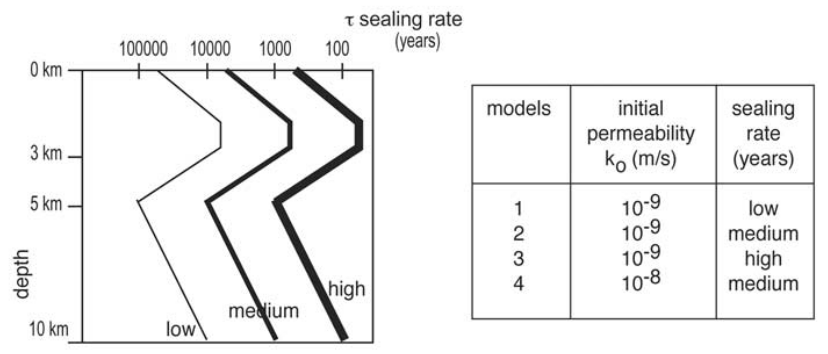
\includegraphics[width=15cm]{python_codes/fieldstone_126/images/grfr03a}\\
{\captionfont 
Left (Fig. 9a): Synthetic variation
in crack sealing rate with depth integrating two superimposed calcite-rich and quartz-rich levels: crack
sealing is modeled with pure calcite between 0 and 3 km, pure quartz between 5 and 10 km and
intermediate behavior between 3 and 5 km. Crack sealing is expressed as the t values (time require in
order to divide the initial porosity by 2.72). Three sets of crack sealing values are derived from this
section: low, medium and high sealing rate profiles.
Right (Fig. 9b): Table of values of the main modeling parameters:
initial permeability $k_0$ and sealing rate. 
The initial porosity along the fault is 10\% (Figures 9c, 10, and 11 of the paper) 
or 1\% (Figures 12 and 13 of the paper).}
\end{center}


\begin{center}
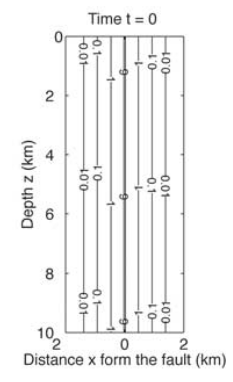
\includegraphics[width=7cm]{python_codes/fieldstone_126/images/grfr03b}\\
{\captionfont Fig. 9c: initial porosity profile.}
\end{center}

I first had an issue with this figure. In the center/fault the porosity
should be $\Phi_0=0.1$ (see Eq.~\eqref{eq:por03}) so how come 
there are isolines 1 on each side of the fault and the fault itself is at 9 (or 6?).
It actually looks like the center value is 10, not 0.1 ... Was it normalised somehow? 
The authors answered: ``
The maximum porosity along the fault is 10\%. 
The porosity is expressed as percentages in figure 9c (and not as volume fraction), 
so 9 on the figure means 9\%.''
The rest of the panels of Fig.~9c,d can be reproduced via Eq.~\eqref{eq:por03} 
(porosity is only a function of time and space).


%%%%%%%%%%%%%%%%%%%%%%%%%%%%%%%%%%%%%%%%%%%%%%%%%%%%%%%%%%%%%%%%
\newpage
\section*{FEM discretisation and code structure}

Based on Fig 9 of the paper the domain is a Cartesian box of 
size $4~\si{\km} \times 10~\si{\km}$ (also clear from paragraph 45). 
In the paper the vertical $z$ axis points down (note that our code will 
not follow this convention and that the axis will be $x,y$ as usual with $y$
pointing upward). 
Note that the domain is in fact $[-2:2]\times[0:10]~\si{\km}$. 
From Eq.~\eqref{eq:por02} and various figures we know that the main 
unknown we are solving for is the overpressure $p$.
The PDE to be solved is the following 
\[
C \upphi_m \frac{\partial p}{\partial t} 
=\frac{\partial}{\partial x} \left( K_x \frac{\partial p}{\partial x} \right) 
+ \frac{\partial}{\partial y} \left( K_y \frac{\partial p}{\partial y} \right)
- \frac{\partial \upphi_m}{\partial t} 
\]
which is a diffusion equation in 2d, with a source term. 
This equation must be supplemented by equations for $K_x(x,y,t)$, $K_y(x,y,t)$, $\upphi_m(x,y,t)$ and 
$\frac{\partial \upphi_m}{\partial t} (x,y,t)$, i.e. Eqs.~\eqref{eq:por06}, 
\eqref{eq:por07}, \eqref{eq:por03}, \eqref{eq:por04}:
\begin{eqnarray}
K_x(x,y,t) &=& \frac{k_0 }{\rho_m g}  \exp\left(-\frac{x}{L}\right) \exp\left(-3\frac{t}{\tau(y)}\right) \nn\\
K_y(x,y,t) &=& 100\frac{k_0 }{\rho_m g}  \exp\left(-\frac{x}{L}\right) \exp\left(-3\frac{t}{\tau(y)}\right) \nn\\
\upphi_m(x,y,t) &=& \upphi_0 \exp (-x/L) \exp (-t/\tau(y)) \nn\\
\frac{\partial \upphi_m}{\partial t}(x,y,t) &=& -\frac{\upphi_0}{\tau(y)} \exp (-x/L) \exp (-t/\tau(y)) \nn
\end{eqnarray}
Finally we will need the parameters $k_0$, $\rho_m$, $g$, $\upphi_0$, $L$, $C$ and the curve $\tau(y)$.
They have all been specified in the text above:

\begin{itemize}
\item $k_0 = 10^{-9}~\si{\meter\per\second}$ or $10^{-8}~\si{\meter\per\second}$
\item $\rho_m=880~\si{\kg\per\cubic\meter}$, 
\item $g=10~\si{\meter\per\square\second}$, 
\item $\rho_{litho}=2800~\si{\kg\per\cubic\meter}$, 
\item $L=100~\si{\meter}$, 
\item $C=10^{-9}~\si{\per\pascal}$.
\item $\phi_0=1\%,10\%$ is a maximum porosity value along the fault, the initial porosity profile shows an
exponential decrease away from the fault
\end{itemize}

%..........................................
\paragraph{Some thoughts about $\tau(z)$}

I have digitized\footnote{\url{https://plotdigitizer.com/app}} Fig.~9a:
\begin{center}
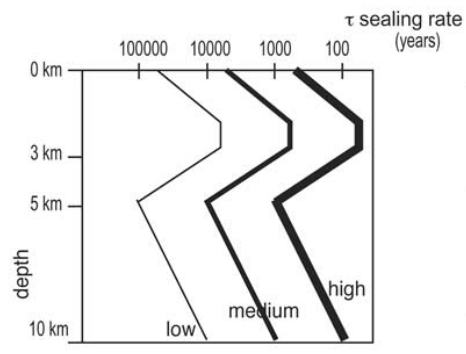
\includegraphics[width=8cm]{python_codes/fieldstone_126/images/grfr03f}
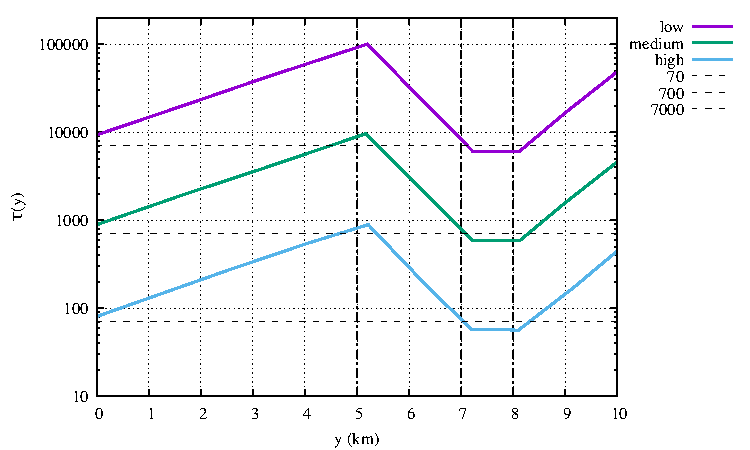
\includegraphics[width=8cm]{python_codes/fieldstone_126/images/tau.pdf}\\
{\captionfont Left: Fig.~9a of the paper; Right: digitized version, note that $y$ is not depth but the
vertical coordinate which points upward.}
\end{center}
When zooming in we see that the original figure is just a drawing 
and serves as an indication rather than 
an accurate representation of the sealing rate $\tau$.
The three broken lines are identical but off by a factor 10.  
Fig.~10 showcases the parameter $\tau_m=70,700,7000~\si{\year}$ which is not discussed in the text
but which seems to correspond to the flat portions of the curves of Fig.~9a (i.e. the minimum value
of $\tau$).
The authors answered: ``Yes the figure 9a is just a schematic drawing i
and serves as an indication rather than an accurate representation of the 
sealing rate $\tau$ and yes the parameter $\tau_m=70,700,7000~\si{\year}$ 
corresponds to the flat portions of the curves of Fig. 9a. We agree that this 
figure could have been more accurate, but the transition values 3 and 5 km 
are the accurate numbers of the transition.''

In the paper we read ``
In the upper crust, we assume the predominance of the calcite rate of crack sealing
at low temperature and pressure while in the deeper crust we
assume the predominance of the rate of crack sealing of the
quartzite at higher temperature and pressure (Renard et al.,2000). 
The depth of transition between these two end-member cases is chosen to be at 3 km.''
Looking at the digitized figure it is obvious the figure is incorrect. The 3km-depth 
line (i.e. the $y=7~\si{\km}$ line) does not align with the transition of the curves.

On page 18 we read ``
For the kinetics of crack sealing, a simplified
variation with depth is used, assuming that the rate of
sealing is controlled by calcite between 0 and 3 km, by
quartz between 5 and 10 km, and by an intermediate
behavior between 3 and 5 km (see Figure 9a). Because of
the uncertainty on the parameters of the calculation the same
profile has been used with three different orders of magnitude 
for the $\tau$ values.
[...] The sealing rates used here were also chosen as fast
as realistic in order to be able to run the calculation for an
acceptable time.
''

In light of all this I have written a single function that returns $\tau$ as a function of $y$
and it corrects the problems highlighted above. 
For the `low' curve: it starts at (0,10000), goes to (5,100000), then to (7,7000), plateaus
until (8,7000) and then goes up to (10,50000).
The other two lines follow the same pattern but their $\tau$ values are a factor 10 and 100 lower.
The Python function is then as follows:
\begin{lstlisting}
def tau_fct(y,srcoeff):
    if y<5.e3:
       val=1e4+y/5e3*(1e5-1e4)
    elif y<7e3:
       val=1e5-(y-5e3)/(7e3-5e3)*(1e5-7000)
    elif y<8e3:
       val=7000
    else:
       val=7000+(y-8000)/(10e3-8e3)*(50000-7000)
    return val*year*srcoeff
\end{lstlisting}
The \lstinline{srcoeff} is either 1 (high sealing rate), 0.1 (medium sealing rate)
or 0.01 (high sealing rate).


%..............................
\paragraph{Initial conditions}

%paragraph 45
Just after an earthquake, the initial condition at $t=0$ is $p=0$ (and consequently 
$\upphi'=0$  and $\rho'=0$).

%..............................
\paragraph{Boundary conditions}

%paragraph 45
The calculation was based on the following boundary conditions: 
\begin{itemize}
\item top: $p=0$;
\item sides:  $\partial p/\partial x =0$ (i.e. $u_x=0$, no flow);
\item bottom: imposed pressure zone scaled
with the fault zone, i.e., $p = g h (\rho_{litho} -\rho_m) e^{-x/L}$.
The maximum value is then $g h (\rho_{litho} -\rho_m) 
=10\cdot 40e3 \cdot(2800-880)=192~\si{\mega\pascal}$.
It is plotted here under: 
\begin{center}
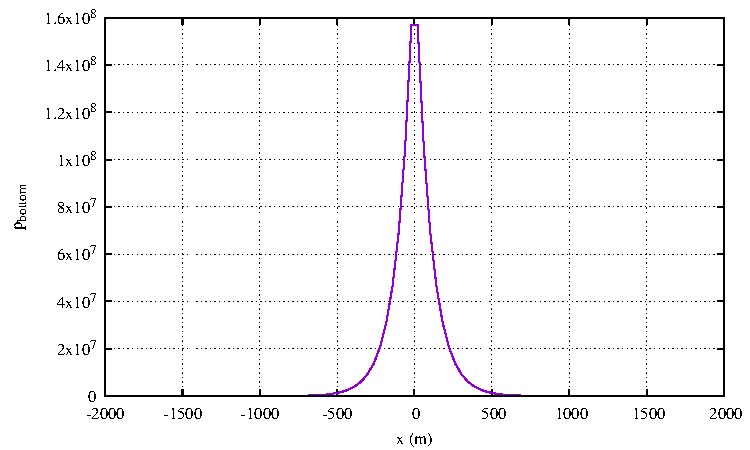
\includegraphics[width=7cm]{python_codes/fieldstone_126/images/pbottom}\\
{\captionfont Pressure imposed at the bottom. Note that for some reason 
gnuplot will not evaluate the functionat x=0 and the peak therefore does not 
reach the 192 MPa value...}
\end{center}

Note that at $x=0$ then the pressure is given by $g h (\rho_{litho} -\rho_m)$
which is in fact $P_{litho}-P_{hydro}$ at the bottom, so that $O_{vp}=p/(P_{litho}-P_{hydro})=1$
at $x=0$ (easy to verify in ParaView). 

\end{itemize}
I suspect the authors to only solve for half the domain (because of symmetry, thereby 
saving computational time) since they 
specify boundary conditions on the fault. Also the expressions for $K_x$ and $K_z$ 
contain the term $\exp(-x/L)$ instead of $\exp(-|x|/L)$.

%..............................
\paragraph{Weak form}

The PDE above is solved by means of the Finite element method, using 
quadratic $Q_2$ elements.
How to establish the weak form of the diffusion equation has been 
carried out in Section~\ref{MMM-ss:hte_fem} of my FieldStone compendium 
document\footnote{See part 1 at \url{https://cedrict.github.io/}.}
so I will not repeat it here. 
The only main difference from the standard diffusion equation for temperature
is that the coefficients and the source term are all space and time dependent.

The discretised weak form is given by
\[
\underbrace{
\left( \int_\Omega \vec{\bN}^T \upphi_m C  \vec{\bN} dV  \right)
}_{\M}
 \cdot \frac{\partial \vec{\cal P}}{\partial t}
+
\underbrace{
\left( \int_\Omega {\bm B}^T \cdot  {\bm K} \cdot {\bm B} dV \right)
}_{{\K}_d}
 \cdot \vec{\cal P}
=
\underbrace{
-
\int_\Omega \vec{\bN}^T  \frac{\partial \upphi_m}{\partial t} dV
}_{\vec{b}}
\]
Since pressure is prescribed on the top and bottom we need not 
care about the surface terms stemming from the integration by parts on these boundaries. 
On the sides we wish to impose $dp/dx$ which is automatically achieved 
by not specifying/coding any boundary term on these parts of the boundaries.

The time derivative can be discretised by means of a simple explicit scheme:
\[
\frac{\partial \vec{\cal P}}{\partial t} \simeq
\frac{ \vec{\cal P}^{t+\delta t} - \vec{\cal P}^t  }{\delta t}
\]
and one then arrives at 
\[
( {\M} + {\K}_d) \cdot \vec{\cal P}^{t+\delta t} = {\M} \cdot \vec{\cal P}^t  + \vec{b}
\]
Of course this approach is not as accurate as the Crank-Nicolson method which we adopt here.
The matrix is symmetric positive definite which is good news.

Note to self: $\M$ actually depends on time, but I although I reevaluate it 
at every point in time and space my time discretisation does not account for this 
time dependency explicitely. Something to revisit?


%...............................
\paragraph{Time step}
In the context of solving pure diffusion equations for temperature in geodynamics 
the time step is limited by 
\[
\delta t \propto \frac{h^2}{\kappa}
\]
where $\kappa$ is the heat diffusivity.
Here at $t=0$ to simplify things, we can compute the equivalent diffusion coefficient:
\[
\kappa \simeq \frac{\max|{\bm K}|}{\Phi_m C} 
\simeq \frac{ 100 k_0/\rho_m g \exp(-x/L) }{\Phi_0 \exp (-x/L) C}
\simeq \frac{ 100 k_0   }{\rho_m g \Phi_0  C}
= \frac{100 \cdot 10^{-9}}{2800 \cdot 10 \cdot 0.1 \cdot 10^{-9}} \simeq 0.0357 m^2/s
\]
Then for $h=100m$ (resolution $40\times 100$), 
\[
\delta t \propto  \frac{100^2}{0.0357} \simeq 280,000 s \simeq 0.0088 yr??!
\]
That value is *very* small. Not quite sure what to think about this right now.
In practice I ended up using much larger values (see here after).

%..........................................
\paragraph{About limiting the overpressure}

In paragraph 43 $P_{hydro}$ is defined by $\vec\nabla P_{hydro} + \rho \vec{g} = \vec{0}$ 
so that in the code we have $P_{hydro}=\rho_m g (L_y -y)$, 
assuming that pressure is zero at the top of the domain. 

Likewise we define $P_{litho}=\rho_{litho} g (L_y -y)$ which 
also means that lithostatic pressure is zero at the top. 

{\color{red} Q2: does this make sense? if so, $O_{vp}$ is ill defined at the top (dividing by zero)?}

{\color{red} Q3: looking at the definition of $O_{vp}$ above an given the boundary conditions $p=0$
at the top, then $O_{vp}=0/0$ at the top?!}

The authors answered: ``In our paper the pore overpressure is $p$ where the total 
fluid pressure $P$ is equal to $p + P_{hydro}$. However, in the paper this $p$ parameter 
is sometime named 'overpressure' and sometime simply 'pressure' which is a bit 
confusing. We did not use the term Ovp but the ratio $p/(Plitho-Phydro)$ cannot reach 1 (see Q4).''

As mentioned earlier the $O_{vp}$ quantity cannot exceed 1. This needs to be 
enforced in an {\it ad hoc} manner. The paper is not exceedly clear as how 
this should be achieved. I repeat the relevant lines of the paper with regards 
to this matter:
``
In our model, we consider a monotonic evolution of the pore pressure, that
is when a region reaches the criterion \eqref{eq:por08} at time $t_{litho}$, it
will not unload later, i.e., $p(x,z,t > t_{litho}) = P_{litho}(z)-P_{hydro}(z)$.
Therefore the boundary of the region that has reached the
lithostatic pressure is a moving pressure-imposed boundary
and the fluid flow inside this region is still evaluated with
equation \eqref{eq:por11}.''

I have therefore implemented a simple rule as follows. After I have solved for $p$
I simply threshold it:
\begin{lstlisting}
for i in range(NP):
    p[i]=min(0.999999*(P_litho[i]-P_hydro[i]),p[i])
\end{lstlisting}
In the code above $p$ is such that it can never exceed $P_{litho}(z)-P_{hydro}(z)$ 
(the 0.99999 coefficient is there for safety -- probably not needed in retrospect) but 
in time $p$ *could* become lower than this quantity again in theory which would violate
$p(x,z,t > t_{litho}) = P_{litho}(z)-P_{hydro}(z)$ recommended in the paper. 
In practice, looking at the points measurements, 
I find that once $p$ has been thresholded it remains at $P_{litho}(z)-P_{hydro}(z)$.

{\color{red} Q4: does my limiter this make sense?}
The authors answered: ``Yes p must be lower than the difference 
$Plitho - Phydro$ (equation 15) it is fine.
Moreover, this condition, which corresponds to a cutoff due to possible 
hydraulic fracturing of the crust is a simplification since it would also 
be necessary to include the strength of the rocks but we decided to neglect this aspect.''



%..............................
\paragraph{Numerical experiments:} From Fig.~9b we see that four models are run:
\begin{itemize}
\item model 1: $k_0=10^{-9}~\si{\meter\per\second}$, low sealing rate
\item model 2: $k_0=10^{-9}~\si{\meter\per\second}$, medium sealing rate
\item model 3: $k_0=10^{-9}~\si{\meter\per\second}$, high sealing rate
\item model 4: $k_0=10^{-8}~\si{\meter\per\second}$, medium sealing rate
\end{itemize}

A potential thing to consider is how much the exponential $\exp(-t/\tau(y))$
influences results: in the following figure I plot $\upphi_m$ as a function of 
$x$ and at different times (assuming $\tau(y)=200$yr for simplicity, corresponding
to 'high' sealing rate, and 2000yr for medium and 20000yr for low).

\begin{center}
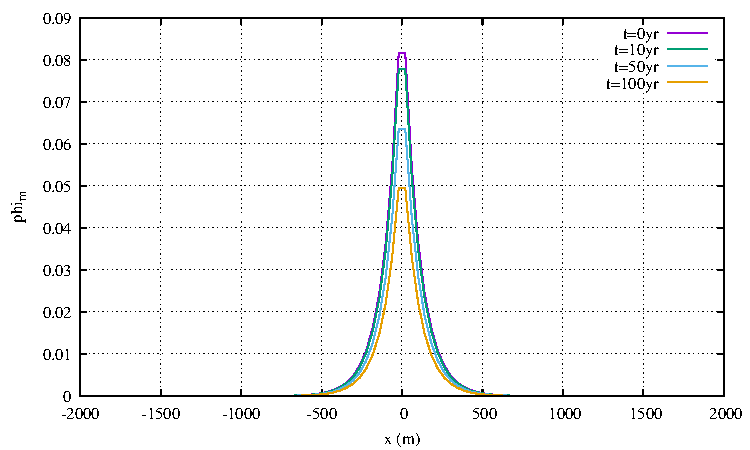
\includegraphics[width=5.7cm]{python_codes/fieldstone_126/images/phi200}
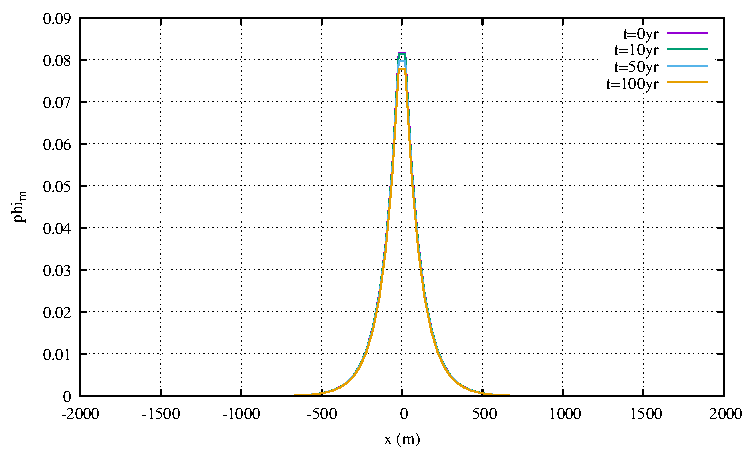
\includegraphics[width=5.7cm]{python_codes/fieldstone_126/images/phi2000}
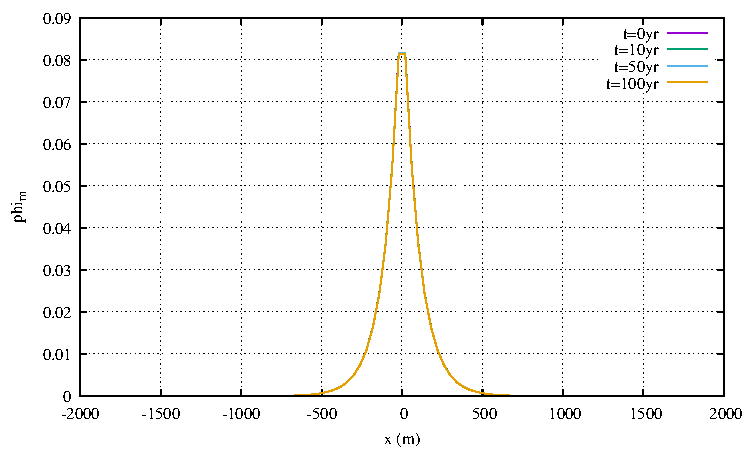
\includegraphics[width=5.7cm]{python_codes/fieldstone_126/images/phi20000}
\end{center}

We see that it changes by less than 50\% in amplitude after 100 years for the 
high sealing rate case, and that it does not change for medium or low.  
This means that $\upphi_m$ barely changes in time and that 
conversely the diffusion coefficient in the form of ${\bm K}$ does not
change in time in most cases. 

The code is written in Python and self contained. It relies on a direct solver
to solve the linear system stemming from the FEM discretisation.
Results are exported in ascii format and in vtu formatted files which can be read by the 
ParaView software\footnote{\url{https://www.paraview.org/}}.


\newpage

%======================================
\section*{Results}

\subsection*{Vizualisation}

In Figs. 10 and 12 the authors show the evolution of the
normalized fluid overpressure $O_{vp} = p/(P_{litho}-P_{hydro})= 
(P- P_{hydro})/(P_{litho} - P_{hydro})$. This quantity is between 0 and 1.

However comparing my results with those of the paper is nearly impossible. Below is the
color scale of the paper next to two similar ones in ParaView. 
\begin{center}
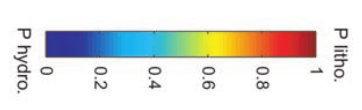
\includegraphics[width=6.4cm]{python_codes/fieldstone_126/images/grfr03_Ovp}\\
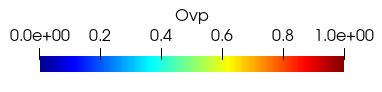
\includegraphics[width=6cm]{python_codes/fieldstone_126/images/jet}\\
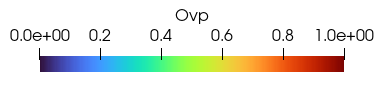
\includegraphics[width=6cm]{python_codes/fieldstone_126/images/turbo}\\
{\captionfont At the top is the colorbar of the paper.
Below is the `Jet' colorbar of ParaView, and at the bottom is 
the 'Turbo' colorbar of Paraview. Looking for example at the light blue color, we see that 
it corresponds to different values of $O_{vp}$ which is obviously
problematic with regards to carrying out a somewhat quantitative comparison.}
\end{center}
Note that the problem regarding appropriate colorscales has since been 
recognised by the community \cite{crsh20}.

I ended up contacting colormaps expert Fabio 
Crameri\footnote{\url{https://www.fabiocrameri.ch/colourmaps/}}
and he was able to create a ParaView-compatible
colormap based on the one found in the paper:
\begin{center}
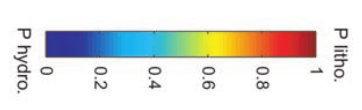
\includegraphics[width=6.6cm]{python_codes/fieldstone_126/images/grfr03_Ovp}\\
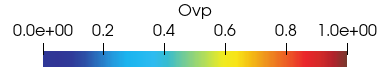
\includegraphics[width=6.4cm]{python_codes/fieldstone_126/images/gratier}
\end{center}
This is obviously a great asset for a thorough comparison. 
I will use this colormap in what follows.


Unless specified the time step $\delta t$ is set to 0.5~\si{\year} for simplicity.
The unfortunate consequence is that the CFL number (based on the Darcy velocity)
is rather large (and close to 1) at high resolutions.
I have however rerun some models with $\delta t=0.25~\si{\year}$ and results 
were virtually unchanged.

At each time step, once $p$ is computed the Darcy velocity $\vec{u}=(u,v)$ is also
computed with $\vec{u}=-\vec\nabla p$. Min/max values of $u,v,p,O_{vp}$ are exported
as a function of time and plotted for the different models.

The evolution of $p$, $u$, $v$ and $O_{vp}$ are also recorded at five points.
The points are $(0,L_y/5)$, $(0,2L_y/5)$, $(0,3L_y/5)$, $(0,4L_y/5)$ and $(L_x/4,7L_y/10)$
as shown on the following figure:

\begin{center}
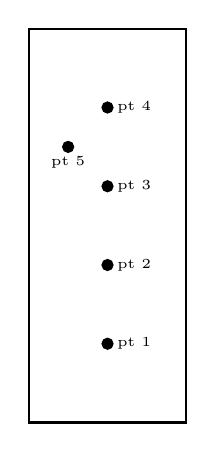
\begin{tikzpicture}
%\draw[fill=gray!23,gray!23](0,0) rectangle (4,7);
%\draw[step=0.5cm,gray,very thin] (0,0) grid (4,7); %background grid
\draw[thick] (1,1) -- (3,1) -- (3,6) -- (1,6) -- cycle  ; 
\filldraw[black] (2,2) circle (2pt) node[anchor=west]{\tiny pt 1};
\filldraw[black] (2,3) circle (2pt) node[anchor=west]{\tiny pt 2};
\filldraw[black] (2,4) circle (2pt) node[anchor=west]{\tiny pt 3};
\filldraw[black] (2,5) circle (2pt) node[anchor=west]{\tiny pt 4};
\filldraw[black] (1.5,4.5) circle (2pt) node[anchor=north]{\tiny pt 5};
\end{tikzpicture}
\end{center}





\newpage
%------------------------------------------------------------------------------
\subsection*{Model 1}

\begin{center}
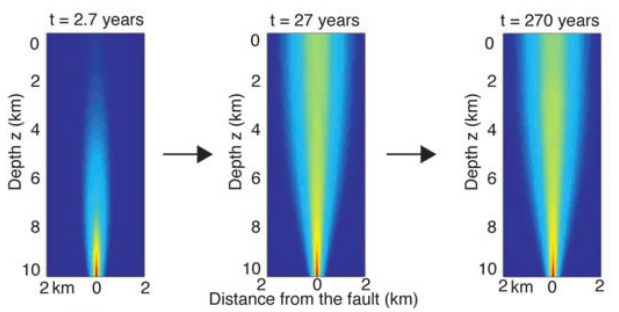
\includegraphics[width=13cm]{python_codes/fieldstone_126/images/grfr03_10a}\\
{\captionfont Fig. 10a from the paper:
Fluid transfer modeling along active crustal faults when integrating pressure solution crack sealing
processes in parallel with inflow of deep lower crust fluids (see Figure 9b); 
The initial porosity along the fault surface is 10\%. Time-dependent
variation is from left to right (from 2.7 to 270 years). 
(a) Model 1, initial permeability $k_0 = 10^{-9} m/s$, low sealing rate; 
overpressure rapidly increases at depth (zone with $O_{vp}$ values = 0.9) then very 
slowly extends to the entire fault zone ($O_{vp}$ values reaching 0.6
after several hundred years). 
}
\end{center}


\begin{center}
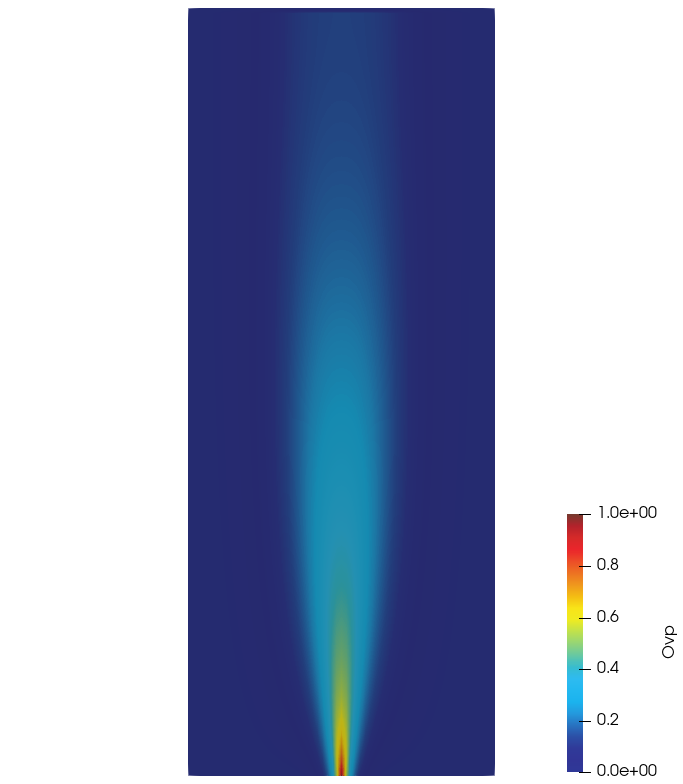
\includegraphics[width=5.cm]{python_codes/fieldstone_126/results/model1/nelx32/Ovp_1.png}
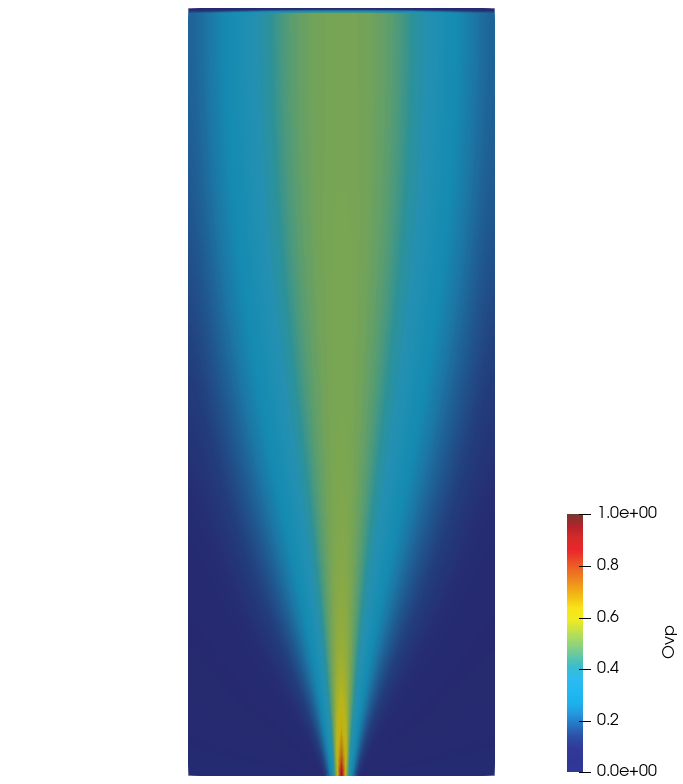
\includegraphics[width=5.cm]{python_codes/fieldstone_126/results/model1/nelx32/Ovp_2.png}
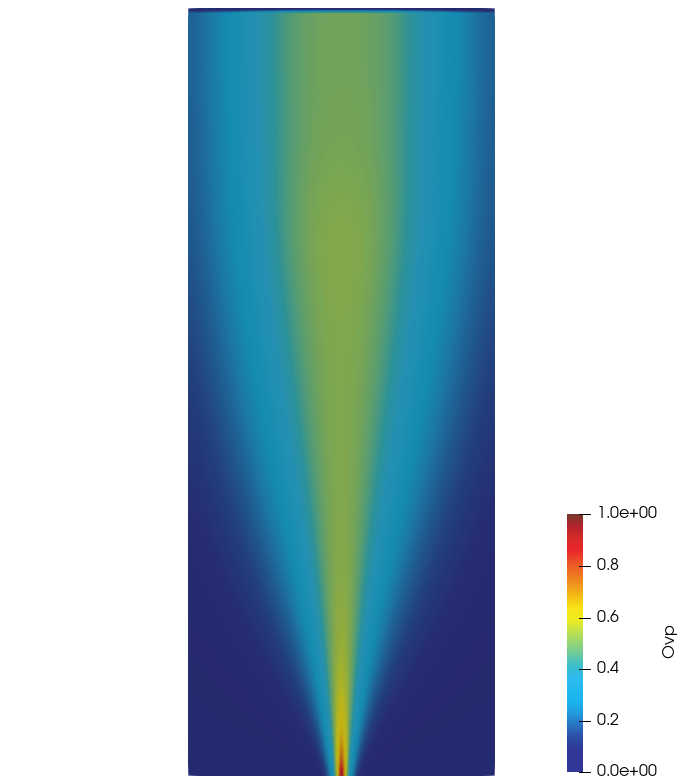
\includegraphics[width=5.cm]{python_codes/fieldstone_126/results/model1/nelx32/Ovp_3.png}\\
{\captionfont Results obtained on $32\times 80$ mesh.}
\end{center}

Looking at my results it looks as if the diffusion in the $x$ direction too strong.
I have therefore (rather arbitrarily) started to reduce $K_x$ by various factors and ultimately 
settled on 2/3.
Results are now:

\begin{center}
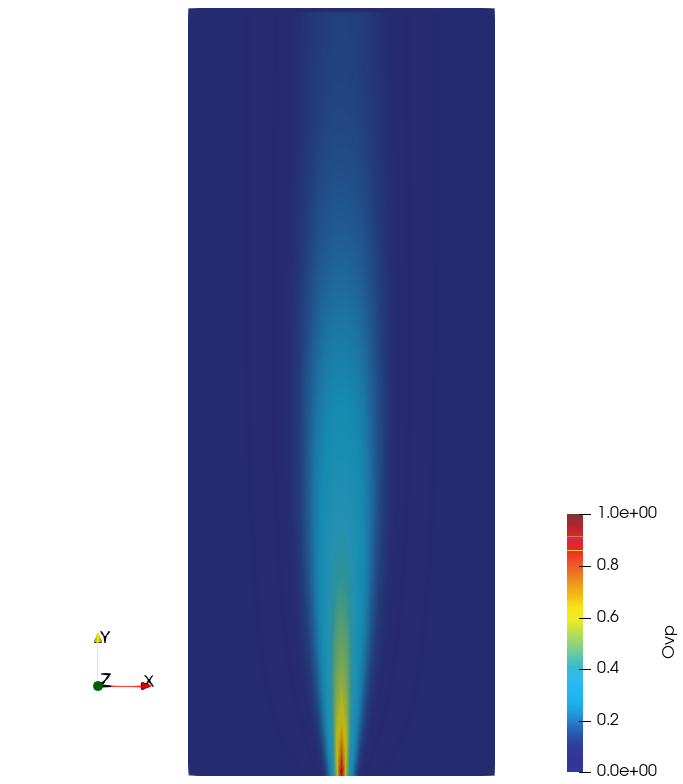
\includegraphics[width=5.cm]{python_codes/fieldstone_126/results/model1_new/Ovp_1.png}
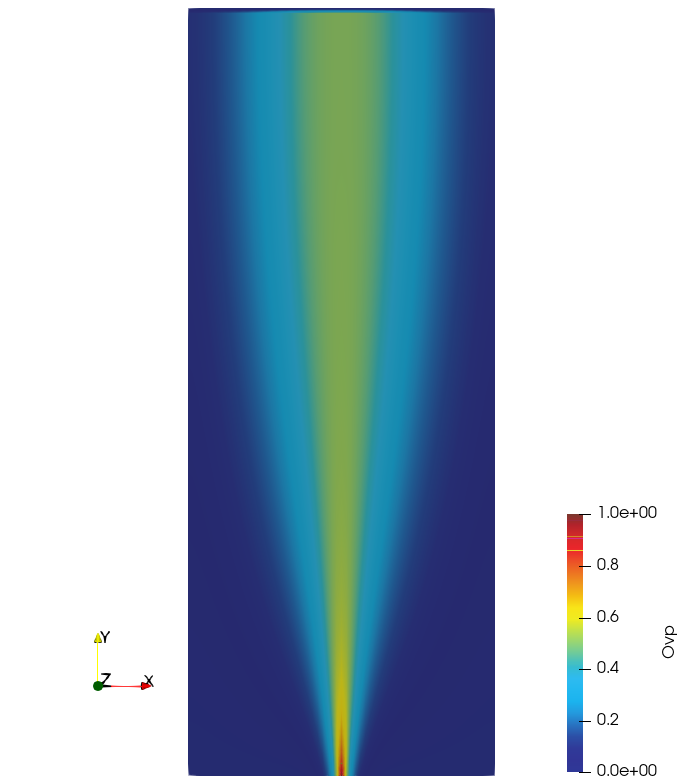
\includegraphics[width=5.cm]{python_codes/fieldstone_126/results/model1_new/Ovp_2.png}
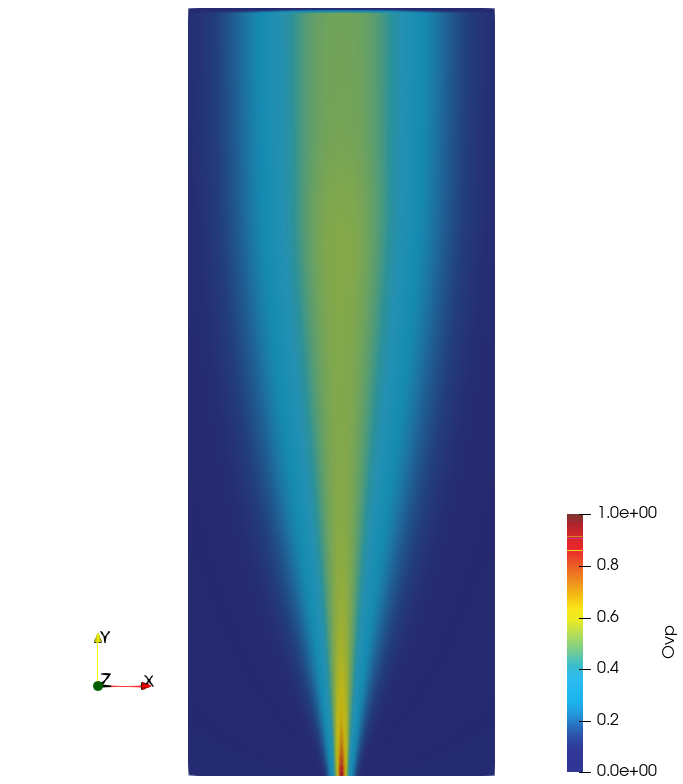
\includegraphics[width=5.cm]{python_codes/fieldstone_126/results/model1_new/Ovp_3.png}\\
{\captionfont Results obtained on $32\times 80$ mesh with $K_x*2/3$.}
\end{center}
My results are then *very* similar to those in the paper.







\newpage
Measurements at the 5 points are shown hereunder:
\begin{center}
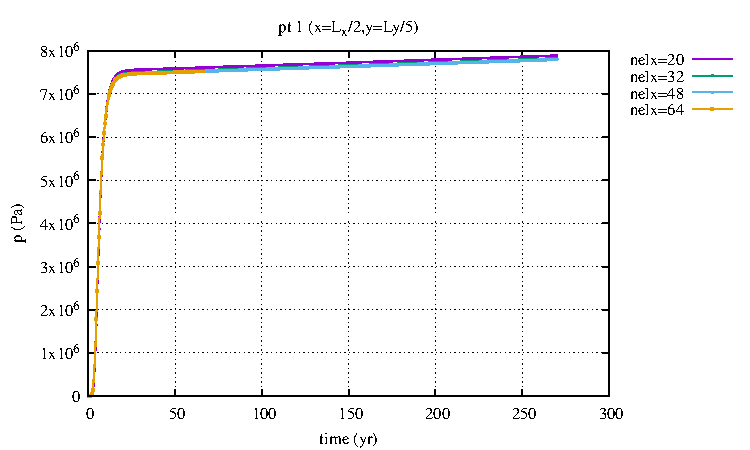
\includegraphics[width=4cm]{python_codes/fieldstone_126/results/model1/pt1_p.pdf}
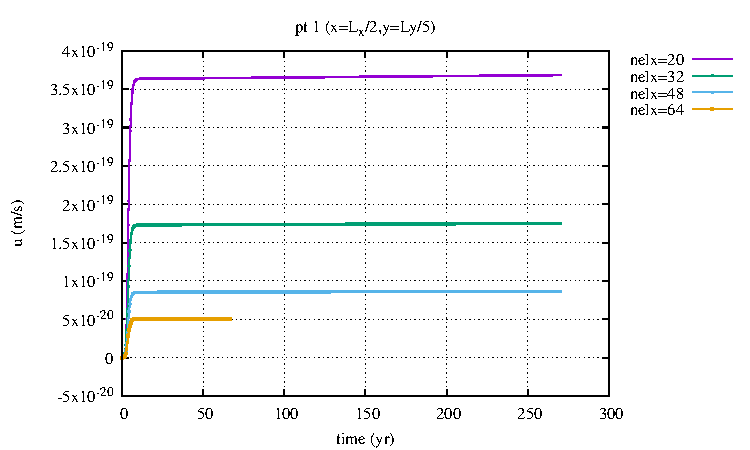
\includegraphics[width=4cm]{python_codes/fieldstone_126/results/model1/pt1_u.pdf}
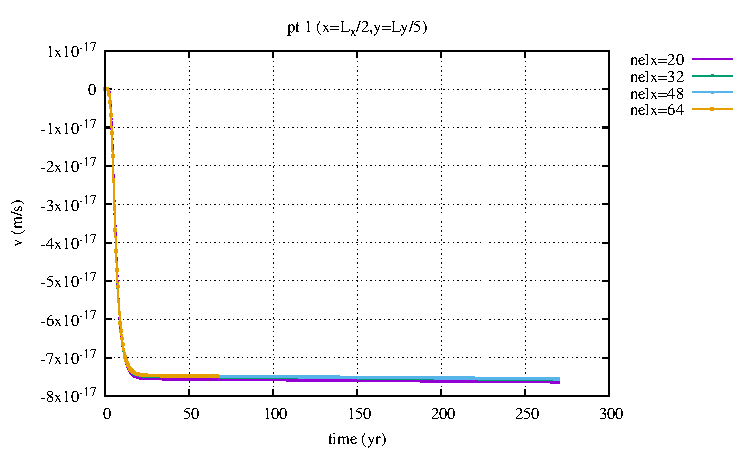
\includegraphics[width=4cm]{python_codes/fieldstone_126/results/model1/pt1_v.pdf}
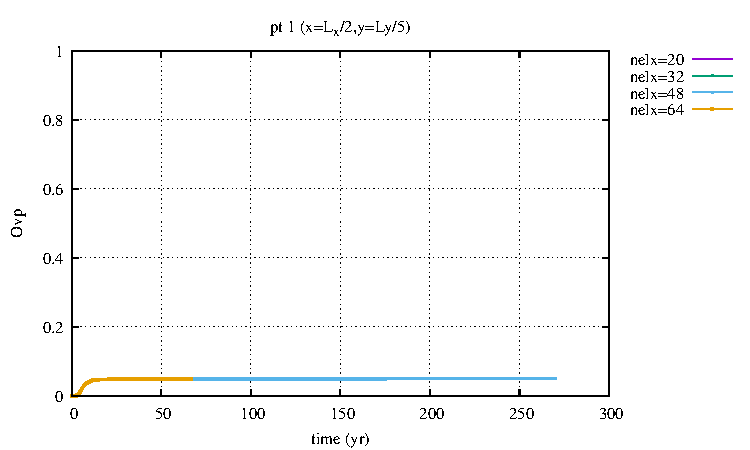
\includegraphics[width=4cm]{python_codes/fieldstone_126/results/model1/pt1_Ovp.pdf}\\
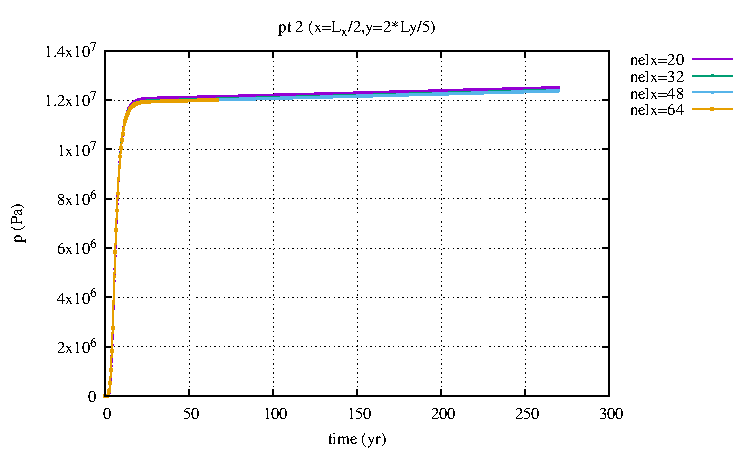
\includegraphics[width=4cm]{python_codes/fieldstone_126/results/model1/pt2_p.pdf}
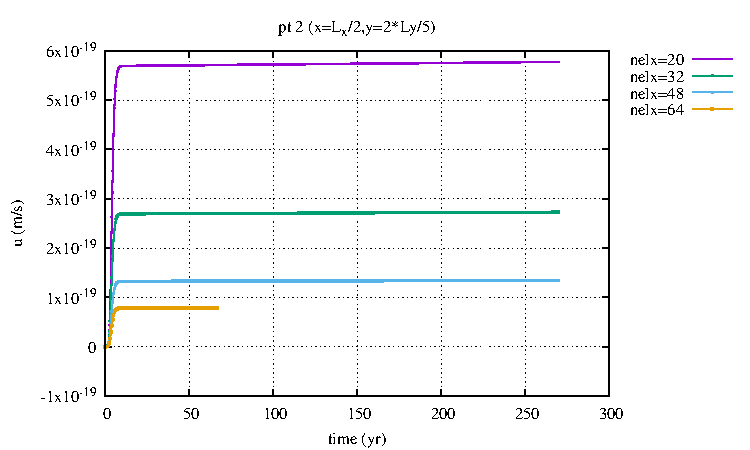
\includegraphics[width=4cm]{python_codes/fieldstone_126/results/model1/pt2_u.pdf}
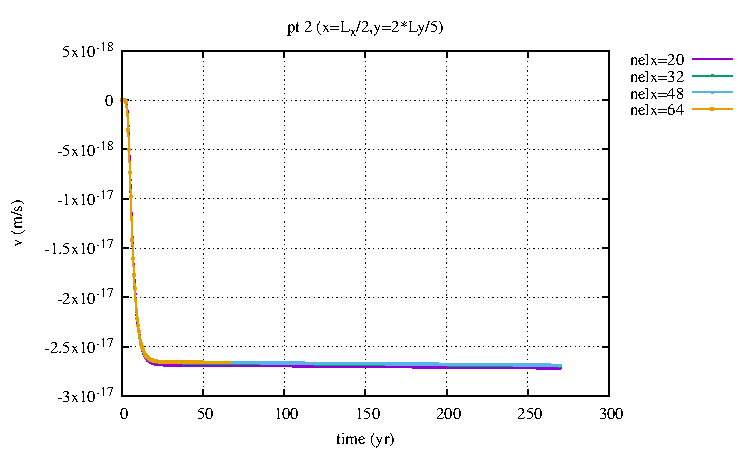
\includegraphics[width=4cm]{python_codes/fieldstone_126/results/model1/pt2_v.pdf}
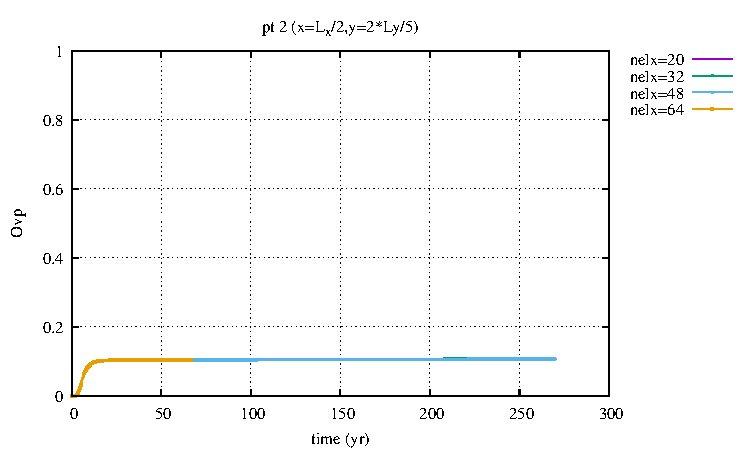
\includegraphics[width=4cm]{python_codes/fieldstone_126/results/model1/pt2_Ovp.pdf}\\
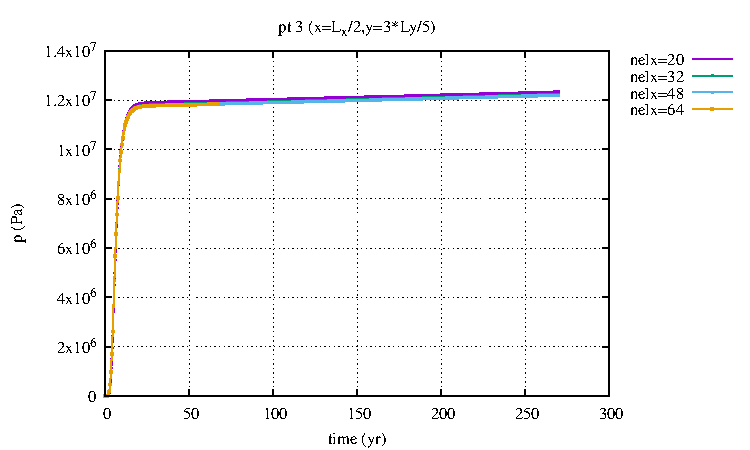
\includegraphics[width=4cm]{python_codes/fieldstone_126/results/model1/pt3_p.pdf}
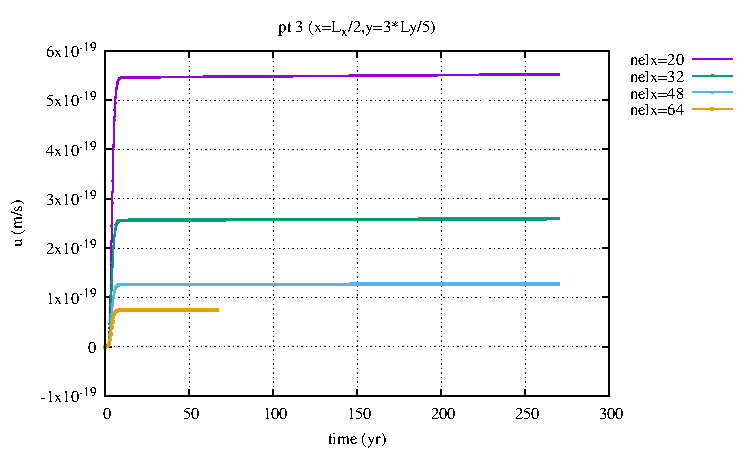
\includegraphics[width=4cm]{python_codes/fieldstone_126/results/model1/pt3_u.pdf}
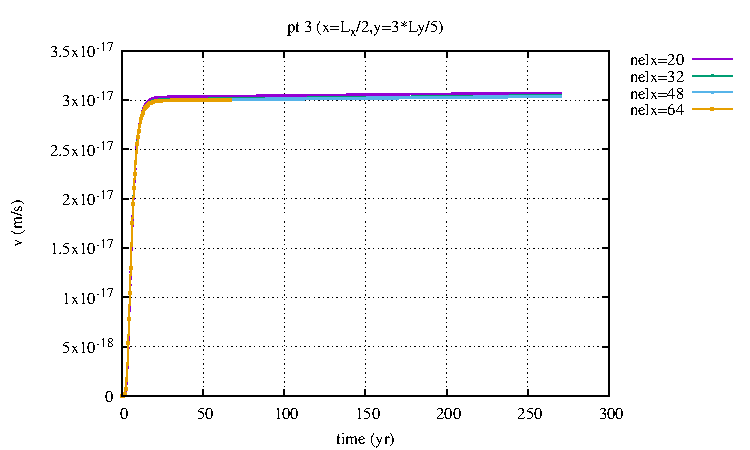
\includegraphics[width=4cm]{python_codes/fieldstone_126/results/model1/pt3_v.pdf}
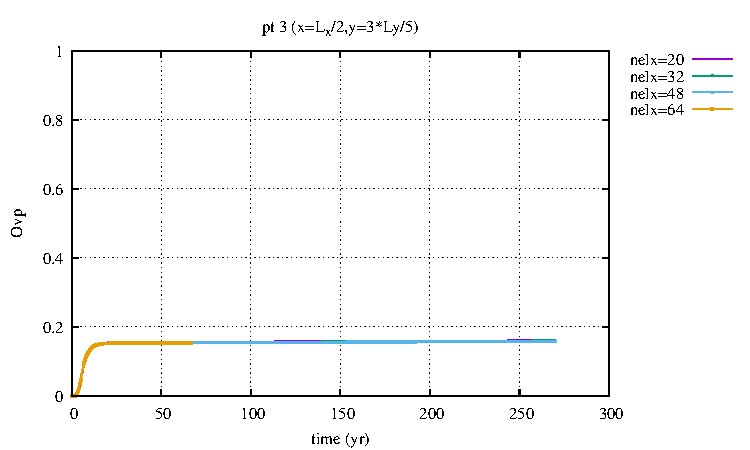
\includegraphics[width=4cm]{python_codes/fieldstone_126/results/model1/pt3_Ovp.pdf}\\
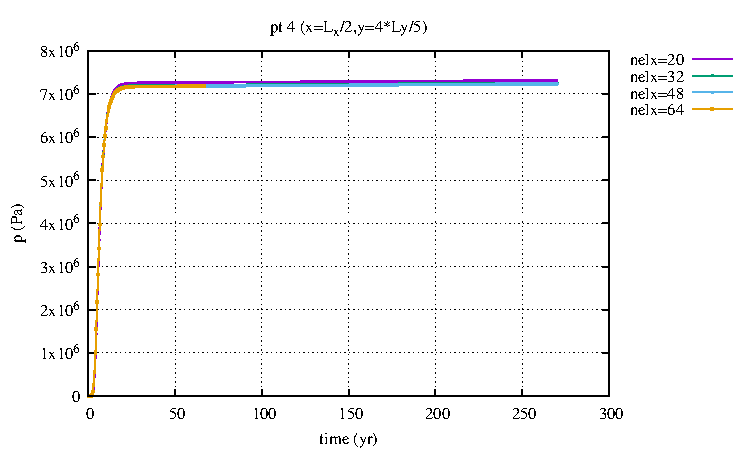
\includegraphics[width=4cm]{python_codes/fieldstone_126/results/model1/pt4_p.pdf}
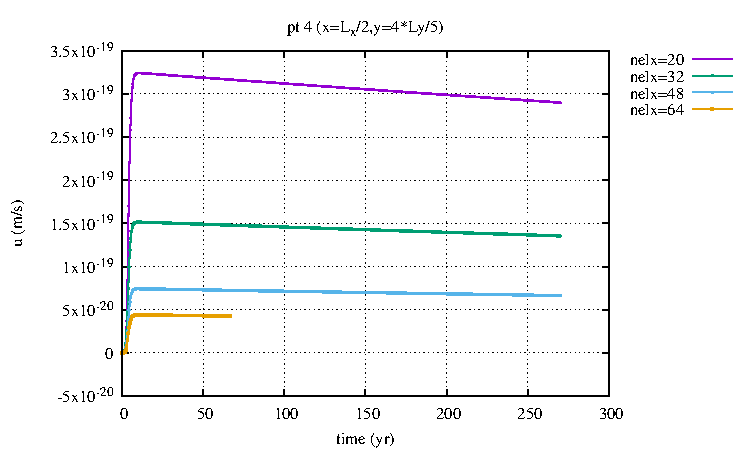
\includegraphics[width=4cm]{python_codes/fieldstone_126/results/model1/pt4_u.pdf}
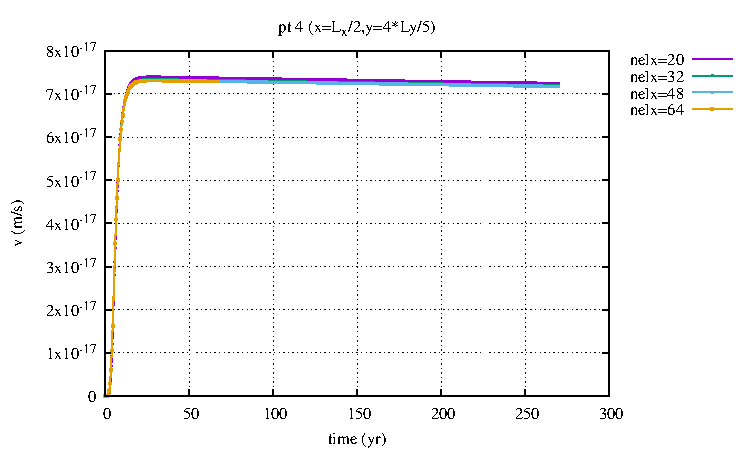
\includegraphics[width=4cm]{python_codes/fieldstone_126/results/model1/pt4_v.pdf}
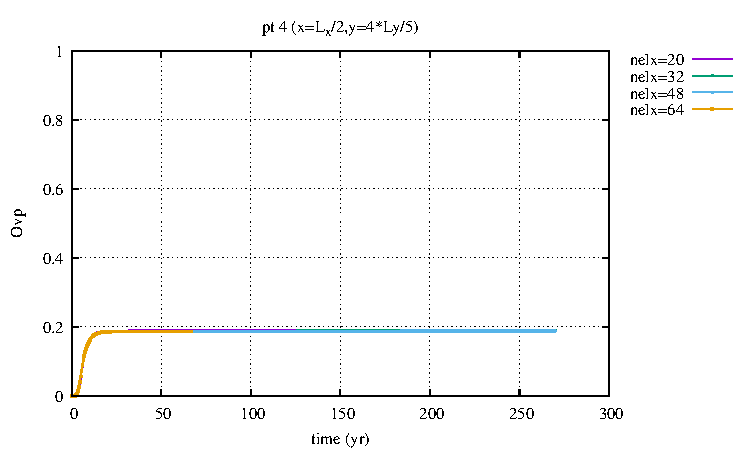
\includegraphics[width=4cm]{python_codes/fieldstone_126/results/model1/pt4_Ovp.pdf}\\
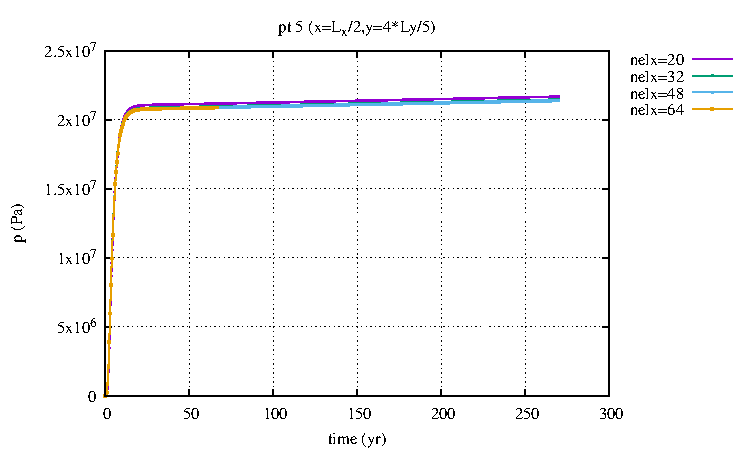
\includegraphics[width=4cm]{python_codes/fieldstone_126/results/model1/pt5_p.pdf}
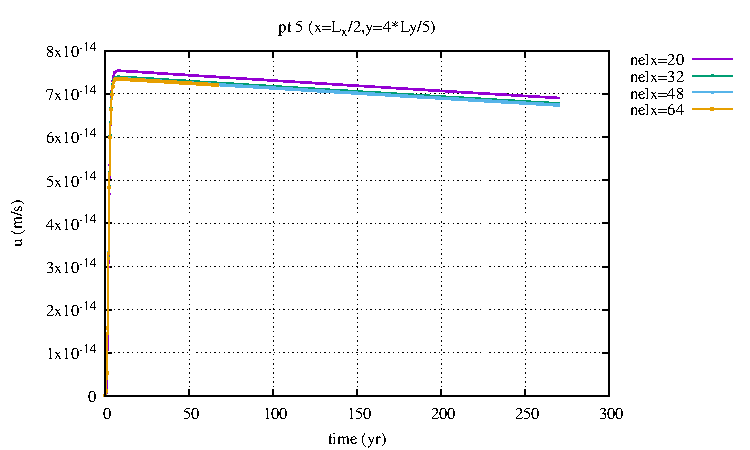
\includegraphics[width=4cm]{python_codes/fieldstone_126/results/model1/pt5_u.pdf}
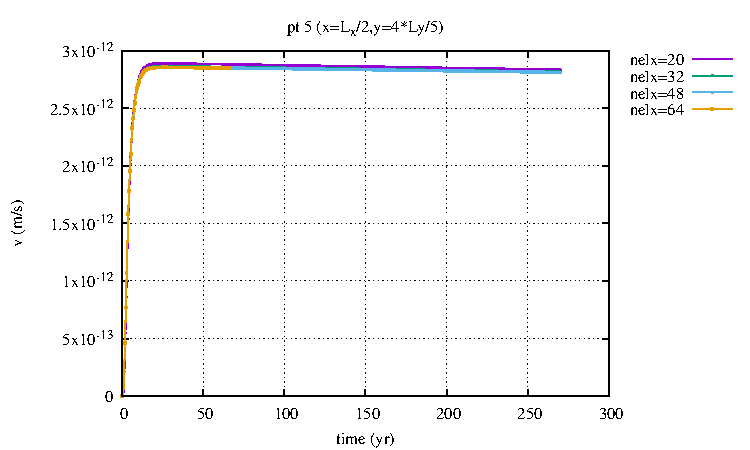
\includegraphics[width=4cm]{python_codes/fieldstone_126/results/model1/pt5_v.pdf}
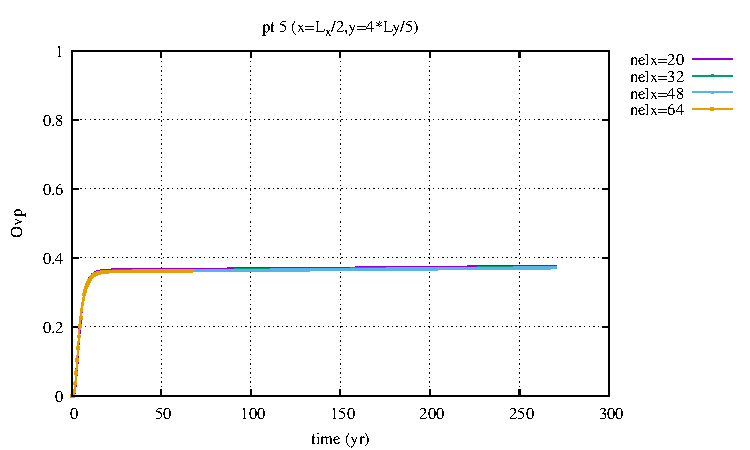
\includegraphics[width=4cm]{python_codes/fieldstone_126/results/model1/pt5_Ovp.pdf}\\
{\captionfont Conclusion: It looks like resolution does not change results much.}
\end{center}

%\begin{center}
%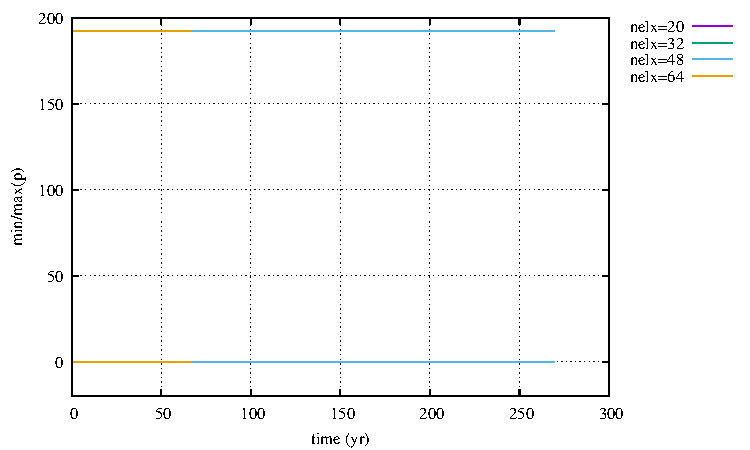
\includegraphics[width=4cm]{python_codes/fieldstone_126/results/model1/stats_p.pdf}
%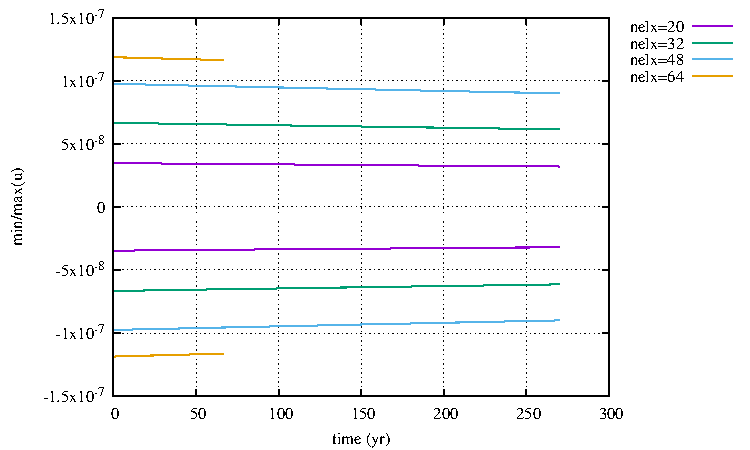
\includegraphics[width=4cm]{python_codes/fieldstone_126/results/model1/stats_u.pdf}
%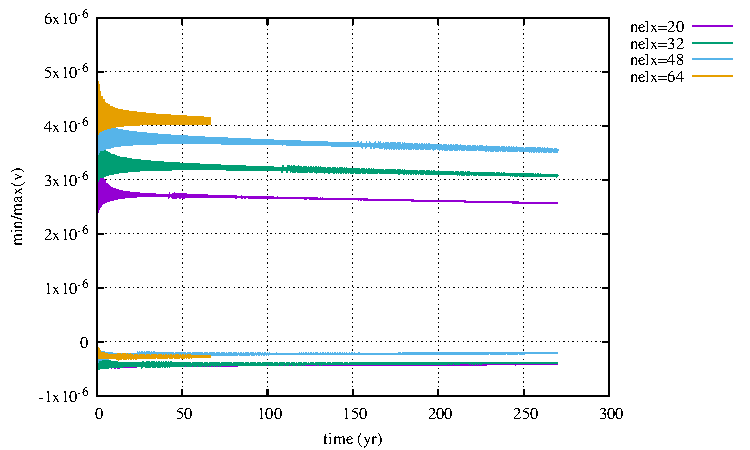
\includegraphics[width=4cm]{python_codes/fieldstone_126/results/model1/stats_v.pdf}
%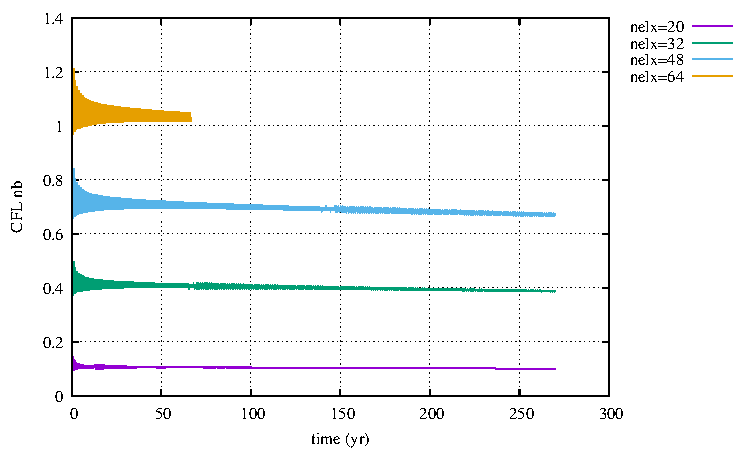
\includegraphics[width=4cm]{python_codes/fieldstone_126/results/model1/cfl.pdf}\\
%\end{center}





\newpage

\begin{center}
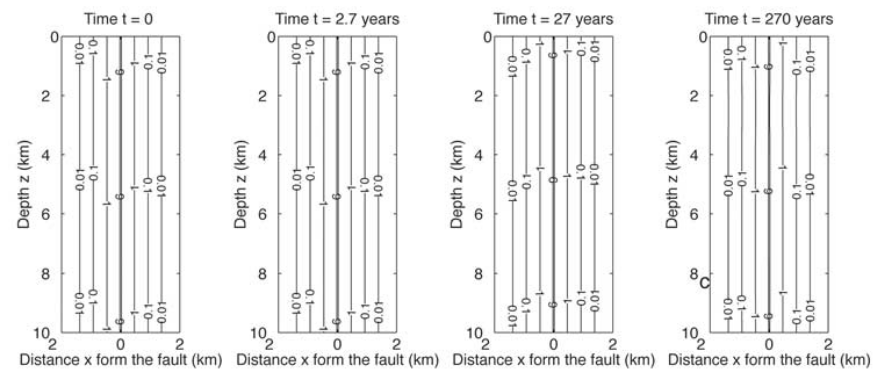
\includegraphics[width=14.7cm]{python_codes/fieldstone_126/images/grfr03c}\\
{\captionfont Fig. 9c of the paper: Evolution of the porosity values with time (t), 
through crustal cross section perpendicular to the fault (located at x=0); 
evolution is obtained with the lowest sealing rate (model 1, Figure 9b),
initial porosity profile}
\end{center}

\begin{center}
\includegraphics[width=4cm]{python_codes/fieldstone_126/results/model1/nelx32/phi_0.png}
\includegraphics[width=4cm]{python_codes/fieldstone_126/results/model1/nelx32/phi_1.png}
\includegraphics[width=4cm]{python_codes/fieldstone_126/results/model1/nelx32/phi_2.png}
\includegraphics[width=4cm]{python_codes/fieldstone_126/results/model1/nelx32/phi_3.png}\\
{\captionfont Evolution of porosity in time.}
\end{center}

We find that for this model $\Phi_m$ does not significantly evolve in time.



\newpage
%------------------------------------------------------------------------------
\subsection*{Model 2}

\begin{center}
\includegraphics[width=13cm]{python_codes/fieldstone_126/images/grfr03_10b}\\
{\captionfont Fig. 10a of the paper:
Model 2, initial permeability $k_0 = 10^{-9} m/s$, medium sealing rate; same fast localized
overpressure development at depth (red zone) slowly extending to the whole fault. However, 
medium sealing rate allows localized overpressure development in the upper part 
of the seismic crust (270 years). 
}
\end{center}

\begin{center}
\includegraphics[width=5.cm]{python_codes/fieldstone_126/results/model2/nelx32/Ovp_1.png}
\includegraphics[width=5.cm]{python_codes/fieldstone_126/results/model2/nelx32/Ovp_2.png}
\includegraphics[width=5.cm]{python_codes/fieldstone_126/results/model2/nelx32/Ovp_3.png}\\
{\captionfont Results obtained on $32\times 80$ mesh.}
\end{center}

Same as in model 1, the results above look as if diffusion 
in the $x$ direction is somewhat to strong,
so $K_x$ is then reduced by a factor 2/3 and results are now:

\begin{center}
\includegraphics[width=5.cm]{python_codes/fieldstone_126/results/model2_new/Ovp_1.png}
\includegraphics[width=5.cm]{python_codes/fieldstone_126/results/model2_new/Ovp_2.png}
\includegraphics[width=5.cm]{python_codes/fieldstone_126/results/model2_new/Ovp_3.png}\\
{\captionfont Results obtained on $32\times 80$ mesh with $K_x*2/3$.}
\end{center}
We obtain *very* similar results as in the paper.






\newpage
%------------------------------------------------------------------------------
\subsection*{Model 3}

\begin{center}
\includegraphics[width=13cm]{python_codes/fieldstone_126/images/grfr03_10c}\\
{\captionfont Fig. 10c of the paper:
Model 3, initial permeability $k_0 =10^{-9} m/s$, high sealing rate; same fast localized overpressure 
development at depth (red zone). However, high sealing rate rapidly develops localized overpressure 
in the upper part of the seismic crust and prevents the outflow of the fluid (before 108 years). }
\end{center}

{\color{red} Q5: based on the successes of models 1\&2, 
I find the first two left panels above somewhat suspicious in the 
light of my results below.}
The authors answered: ``We agree that in this case there is a difference between our 
figure and your results. We do not have an explanation, and we cannot exclude an error 
on how we reported the times on these two panels.''


\begin{center}
\includegraphics[width=4cm]{python_codes/fieldstone_126/results/model3/nelx32/Ovp_1.png}
\includegraphics[width=4cm]{python_codes/fieldstone_126/results/model3/nelx32/Ovp_2.png}
\includegraphics[width=4cm]{python_codes/fieldstone_126/results/model3/nelx32/Ovp_3.png}
\includegraphics[width=4cm]{python_codes/fieldstone_126/results/model3/nelx32/Ovp_4.png}\\
{\captionfont Results obtained on $32\times 80$ mesh.}
\end{center}

Same as in model 1, $K_x$ is then reduced by a factor 2/3 and results are now:

\begin{center}
\includegraphics[width=4.cm]{python_codes/fieldstone_126/results/model3_new/Ovp_1.png}
\includegraphics[width=4.cm]{python_codes/fieldstone_126/results/model3_new/Ovp_2.png}
\includegraphics[width=4.cm]{python_codes/fieldstone_126/results/model3_new/Ovp_3.png}
\includegraphics[width=4.cm]{python_codes/fieldstone_126/results/model3_new/Ovp_4.png}\\
{\captionfont Results obtained on $32\times 80$ mesh with $K_x*2/3$.}
\end{center}
We again obtain *very* similar results as in the paper.



\newpage
Measurements at the 5 points are shown hereunder:
\begin{center}
\includegraphics[width=4cm]{python_codes/fieldstone_126/results/model3/pt1_p.pdf}
\includegraphics[width=4cm]{python_codes/fieldstone_126/results/model3/pt1_u.pdf}
\includegraphics[width=4cm]{python_codes/fieldstone_126/results/model3/pt1_v.pdf}
\includegraphics[width=4cm]{python_codes/fieldstone_126/results/model3/pt1_Ovp.pdf}\\
\includegraphics[width=4cm]{python_codes/fieldstone_126/results/model3/pt2_p.pdf}
\includegraphics[width=4cm]{python_codes/fieldstone_126/results/model3/pt2_u.pdf}
\includegraphics[width=4cm]{python_codes/fieldstone_126/results/model3/pt2_v.pdf}
\includegraphics[width=4cm]{python_codes/fieldstone_126/results/model3/pt2_Ovp.pdf}\\
\includegraphics[width=4cm]{python_codes/fieldstone_126/results/model3/pt3_p.pdf}
\includegraphics[width=4cm]{python_codes/fieldstone_126/results/model3/pt3_u.pdf}
\includegraphics[width=4cm]{python_codes/fieldstone_126/results/model3/pt3_v.pdf}
\includegraphics[width=4cm]{python_codes/fieldstone_126/results/model3/pt3_Ovp.pdf}\\
\includegraphics[width=4cm]{python_codes/fieldstone_126/results/model3/pt4_p.pdf}
\includegraphics[width=4cm]{python_codes/fieldstone_126/results/model3/pt4_u.pdf}
\includegraphics[width=4cm]{python_codes/fieldstone_126/results/model3/pt4_v.pdf}
\includegraphics[width=4cm]{python_codes/fieldstone_126/results/model3/pt4_Ovp.pdf}\\
\includegraphics[width=4cm]{python_codes/fieldstone_126/results/model3/pt5_p.pdf}
\includegraphics[width=4cm]{python_codes/fieldstone_126/results/model3/pt5_u.pdf}
\includegraphics[width=4cm]{python_codes/fieldstone_126/results/model3/pt5_v.pdf}
\includegraphics[width=4cm]{python_codes/fieldstone_126/results/model3/pt5_Ovp.pdf}\\
{\captionfont Conclusion: It looks like resolution does not change results much.}
\end{center}

\begin{center}
\includegraphics[width=4cm]{python_codes/fieldstone_126/results/model3/stats_p.pdf}
\includegraphics[width=4cm]{python_codes/fieldstone_126/results/model3/stats_u.pdf}
\includegraphics[width=4cm]{python_codes/fieldstone_126/results/model3/stats_v.pdf}
\includegraphics[width=4cm]{python_codes/fieldstone_126/results/model3/cfl.pdf}\\
\end{center}


\newpage


\begin{center}
\includegraphics[width=14cm]{python_codes/fieldstone_126/images/grfr03d}\\
{\captionfont Fig. 9d: same as Fig. 9c, but evolution is 
obtained with the highest sealing rate (model 3, Figure 9b).}
\end{center}

\begin{center}
\includegraphics[width=4cm]{python_codes/fieldstone_126/results/model3/nelx32/phi_1.png}
\includegraphics[width=4cm]{python_codes/fieldstone_126/results/model3/nelx32/phi_2.png}
\includegraphics[width=4cm]{python_codes/fieldstone_126/results/model3/nelx32/phi_3.png}
\includegraphics[width=4cm]{python_codes/fieldstone_126/results/model3/nelx32/phi_4.png}\\
{\captionfont Evolution of porosity in time.}
\end{center}






\newpage
%------------------------------------------------------------------------------
\subsection*{Model 4}

\begin{center}
\includegraphics[width=13cm]{python_codes/fieldstone_126/images/grfr03_10d}\\
{\captionfont Fig. 10d of the paper:
Model 4, initial permeability $k_0 = 10^{-8} m/s$, 
medium sealing rate; same fast localized overpressure
development at depth (red zone) rapidly extending to the whole fault after some years, 
contrary to model 2. However, even with the effect of medium sealing rate values, 
localized overpressure finally develops in the upper part of the seismic crust as in model 2 (270 years).
}
\end{center}

\begin{center}
\includegraphics[width=5.cm]{python_codes/fieldstone_126/results/model4/nelx32/Ovp_1.png}
\includegraphics[width=5.cm]{python_codes/fieldstone_126/results/model4/nelx32/Ovp_2.png}
\includegraphics[width=5.cm]{python_codes/fieldstone_126/results/model4/nelx32/Ovp_3.png}\\
{\captionfont Results obtained on $32\times 80$ mesh.}
\end{center}

Same as in other models, $K_x$ is then reduced by a factor 2/3 and results are now:

\begin{center}
\includegraphics[width=5.cm]{python_codes/fieldstone_126/results/model4_new/Ovp_1.png}
\includegraphics[width=5.cm]{python_codes/fieldstone_126/results/model4_new/Ovp_2.png}
\includegraphics[width=5.cm]{python_codes/fieldstone_126/results/model4_new/Ovp_3.png}\\
{\captionfont Results obtained on $32\times 80$ mesh with $K_x*2/3$.}
\end{center}
We again obtain *very* similar results as in the paper.




\newpage

Conclusions and thoughts:

\begin{itemize}
\item my replication seems to be reasonably successful
\item I still have a few questions about some algorithmic choices (especially the 
overpressure limiter)
\item despite these early successes the code should be benchmarked thoroughly 
with manufactured solutions (diffusion, time derivative, calculation 
of pressure derivatives, etc ...) before any result can be part of a publication. 
\item I am not sure how to choose the time step $\delta t$
\item there are velocity oscillations at the beginning that I have not investigated (dt too big?)
\item I could build a Finite difference version of the code too (MSc thesis exercise?).
Based on all I have learned building the FEM code it would nto take long.
\item my results match the paper provided the $K_x$ coefficient is lessened by a factor (approx.) 2/3.
This could point to a bug in the original code? The authors answered:
``We wonder whether this difference might be due to the simplification of the equation 
linking permeability and porosity, see comment above about equation \eqref{eq:por05}.''
\item I have not looked at fig 11 yet : to do !
\item I could extend the code to use $Q_1$ elements.
\item stretch mesh towards the middle?
\end{itemize} 


